\documentclass[12pt]{article}
\usepackage[a4paper, total={7.5in, 11in}]{geometry}
%\usepackage{array}
\usepackage{graphicx, subfig, wrapfig, fancyhdr, lastpage, multicol ,color,arydshln,makecell}
\newcommand\headerMe[2]{\noindent{}#1\hfill#2}
\usepackage[mathscr]{euscript}
\usepackage{tabularray}

\setlength{\columnseprule}{1pt}
\def\columnseprulecolor{\color{blue}}


\pagestyle{fancy}
\fancyhf{}

\cfoot{ \vspace{-0.8cm}\em{Page \thepage \hspace{1pt} / \pageref{LastPage}}}
\begin{document}

\headerMe{Royaume du Maroc}{année scolaire \emph{2022-2023}}\\
\headerMe{Ministère de l'Éducation nationale, }{  Professeur :\emph{Zakaria Haouzan}}\\
\headerMe{du Préscolaire et des Sports}{Établissement : \emph{Lycée SKHOR qualifiant}}\\
\vspace{-1cm}
\begin{center}
Devoir Surveillé  N°1 \\
    2ème année baccalauréat Sciences physiques\\
Durée 2h00
\\
    \vspace{.2cm}
\hrulefill
\Large{Chimie 7pts - 55min}
\hrulefill\\

    %\emph{Les deux parties sont indépendantes}
\end{center}
%end Headerss------------------------
%__________________Chimie ______________________-
%%%%%%%+_+_+_+_+_+_+_+_+_Partie1

 \section*{Suivi temporel d’une transformation chimique par la conductimétrie \dotfill(7pts) }
\begin{wrapfigure}{r}{0.16\textwidth}
	\vspace{-1.2cm}
\begin{center}
  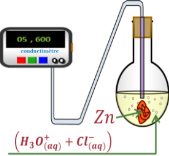
\includegraphics[width=0.16\textwidth]{./img/chimie01.png}
\end{center}
\end{wrapfigure}


Pour étudier la cinématique de la réaction de l’acide chlorhydrique avec le zinc , on introduit dans un
ballon de volume V constant , une masse $m = 1, 04g$ de zinc en poudre $Zn_{(s)}$ et on y verse à l’instant
$t_0$=$0min$ un volume $V_A$=$80mL$ d’une solution aqueuse d’acide chlorhydrique ($H_3O^+_{(aq)} + Cl^-_{(aq)}$) de concentration $C_A$=$0,5mol/L$.

\begin{wrapfigure}[1]{r}{0.5\textwidth}
	\vspace{0.5cm}
\begin{center}
  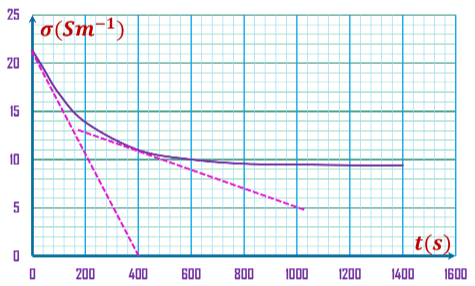
\includegraphics[width=0.5\textwidth]{./img/chimie02.png}
\end{center}
\end{wrapfigure}


L’équation de réaction est : $$2H_3O^+_{(aq)} + Zn_{(s)} \rightarrow {Zn^{2+}}_{(aq)} + {H_2}_{(g)} + 2H_2O_{(l)}$$

On mesure à chaque instant t la conductivité $\sigma(t)$de la solution à l’aide d’un
conductimètre . L’ensembles des résultats de cette expérience permet de tracer
la courbe ci-contre qui représente l’évolution de la conductivité $\sigma(t)$
de la solution en fonction du temps .


\begin{tabular}{c|l}
	0,5  & \makecell[l]{ \textbf{1. }Calculer les quantités de matière\\initiales des réactifs.}\\
	0,5  & \makecell[l]{ \textbf{2. }Dresser le tableau d’avancement de\\cette réaction. }\\
	0,5 & \makecell[l]{ \textbf{3. }Calculer la valeur de l’avancement\\maximal $x_{max}$ de la\\réaction , et déduire le réactif limitant.}\\ 
	0,25 & \makecell[l]{ \textbf{4. }Expliquer la diminution de la\\conductivité mesurée  \\au cours de la transformation chimique.}\\
	1	& \makecell[l]{ \textbf{5. }Montrer que la conductivité du\\ 
	mélange à un instant $t$ est :$\sigma$=$21,30 - 7,42.10^2x$ $(S.m^{-1})$}\\
		1,25 & \makecell[l]{ \textbf{6. }Calculer la composition du système à l’instant $t = 400s$ et déduire le volume  de $H_2$ formé à\\cet instant.}\\
		1 & \makecell[l]{\textbf{7. }Trouver l’expression de v la vitesse volumique en fonction de V et $\frac{d\sigma}{dt}$.Calculer sa valeur\\aux instants $t$=$0s$  et $t$=$400s$ . Expliquer le résultat . }\\
		0,25 &  \textbf{8. } Déterminer en justifiant la réponse le temps de demi-réaction $t_{1/2}$.\\
		0,25 & \makecell[l]{ \textbf{9. } Comment évolue la vitesse de réaction au cours du temps ? Donner une interprétation de \\cette variation en envisageant un facteur cinétique.}\\
		1.5 & \makecell[l]{ \textbf{10. } On refait la même expérience dans les même conditions mais avec 
	une solution de l’acide \\chlorhydrique de concentration $C_A'$=$0, 25mol/L$.\\
	Tracer , en justifiant , sur le même courbe précédente , l’allure de la courbe obtenue dans ce cas.}

\end{tabular}
\begin{center}
\textbf{\underline{ Données : } }

\begin{itemize}
	\item La masse molaire de Zinc: $M(Zn) = 65,4g/mol$.
	\item Le volume molaire $V_m = 25L/mol$
	\item Les conductivités molaire ioniques : 

		$\lambda_{H_3O^+}=34,98 mS.m^2.mol^{-1}$ ; $ \lambda_{Zn^{2+}}=10,56mS.m^2.mol^{-1}$ ; $\lambda_{Cl^-}=7,63 mS.m^2.mol^{-1}$
\end{itemize}

\end{center}



%\hrulefill
%\Large{Physique 13pts/78min}
%\hrulefill\\
\begin{center}
    %\vspace{.60cm}
\hrulefill
\Large{Physique 13pts - 65min}
\hrulefill\\
    \emph{Les  parties sont indépendantes}
\end{center}

\vspace{-1cm}
\section*{Partie 1 :  le mouvement des vagues .......(3pts)}
\vspace{-0.4cm}

\begin{wrapfigure}[2]{r}{0.19\textwidth}
  \begin{center}
	  \vspace{-2cm}
	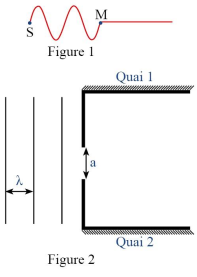
\includegraphics[width=0.19\textwidth]{./img/ex6.png}
  \end{center}
\end{wrapfigure}
On considère que les ondes se propageant à la surface des eaux des mers sont progressives et
sinusoïdales de période T = 7 s.

\begin{tabular}{c|l}
 1 &\textbf{1. }L’onde étudiée est-elle longitudinale ou transversale ? Justifier.\\

 1& \makecell[l]{\textbf{2. }Calculer V, la vitesse de propagation de ces ondes, sachant
 que la \\distance séparant deux crêtes consécutives est d = 70 m.}\\

	 1 & \makecell[l]{\textbf{3. }Les ondes arrivent à un portail de largueur $a = 60 m$ situé entre
	 deux\\quais d’un port (Figure 2). Recopier le schéma de la figure 2, et représenter dessus\\les ondes après la traversée du portail, \\et donner le nom du phénomène observé. puis Calculer $\lambda$}\\
\end{tabular}
\section*{Partie 2 :  Propagation d’une onde ultrasonore dans l’air \dotfill(5pts)}
\begin{wrapfigure}[3]{r}{0.29\textwidth}
  \begin{center}
	  \vspace{-1.5cm}
	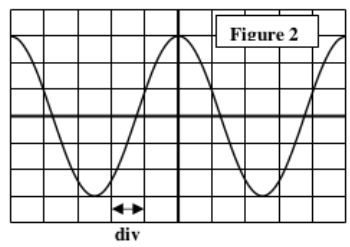
\includegraphics[width=0.29\textwidth]{./img/ex7_1.png}
  \end{center}
\end{wrapfigure}


Pour étudier la propagation des ondes ultrasonores dans l’eau, on utilise un émetteur E et R un récepteur



\begin{tabular}{c|l}
1 & \textbf{1. }Définir une onde mécanique progressive.\\

1 & \makecell[l]{ \textbf{2. }L’onde ultrasonore est-elle une onde longitudinale ou \\transversale ? Justifier la réponse.} \\
1& \makecell[l]{\textbf{3. }Ecrire la relation entre la longueur d’onde $\lambda$, la fréquence N des \\ultrasons et sa célérité de propagation dans un milieu quelconque.}\\
 & \makecell[l]{ \textbf{4. }La courbe de la figure 2 représente les variations de la tension aux bornes du récepteur R, la \\sensibilité horizontale est $S_h=2\mu{s}/div$.}\\
1& \textbf{4.1. }Déterminer graphiquement la valeur de la période T de l’onde reçus par le récepteur R.\\

1 & \makecell[l]{ \textbf{4.2. }Déterminer la valeur $\lambda$ de la longueur d’onde sachant que la vitesse de propagation de l’onde \\sonore dans l’aire est : $V_{air}=340m/s$.}\\
\end{tabular}
\section*{Partie 3 : Étude du phénomène ondulatoire. \dotfill(5pts) }
\begin{wrapfigure}[6]{r}{0.29\textwidth}
  \begin{center}
	  \vspace{-1.5cm}
	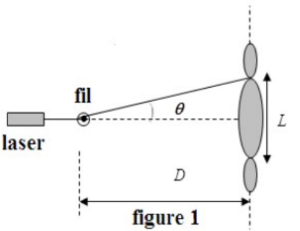
\includegraphics[width=0.29\textwidth]{./img/diff.png}
  \end{center}
\end{wrapfigure}


On réalise une expérience en utilisant un LASER, un fil de diamètre a et un écran. Le dispositif est
représenté ci-dessous (figure 1) :
Les mesures de diamètre du fil a, de la distance du fil à l’écran D
et de la largeur de la tache lumineuse centrale L conduisent
aux résultats suivants : $a = 0,200mm$ et $D=2,00m$ ; $L=12,6mm$.

\begin{tabular}{c|l}
	1 & \makecell[l]{\textbf{1. }Quel est le nom du phénomène observé et déduire la nature de \\la lumière  ?}\\
	0,5	&\makecell[l]{\textbf{2. } a l’aide de la figure 1, Etablir la relation entre $\theta$, L et D\\on supposera $\theta$ est suffisamment petit pour considérer $tan(\theta) = \theta$ avec $\theta$ exprimé en radian.}\\
		0,5& \makecell[l]{\textbf{3. }En utilisant les résultats des mesures, calculer la valeur de l’angle $\theta$ en radians.}\\

	0,5 &\makecell[l]{\textbf{4. }Donner la relation qui lie les grandeurs $\theta$ (écart angulaire), $\lambda$ (longueur d’onde de la
lumière)\\et a (diamètre du fils). Préciser les unités (dans le système international) respectives de ces\\grandeurs physiques.}\\
	0,5 &\makecell[l]{\textbf{5. }Calculer la valeur de la longueur d’onde $\lambda$. Est-ce qu’elle appartient au domaine visible?\\justifier.}\\

	2 &\makecell[l]{\textbf{6. }Indiquer, en justifiant comment varie L lorsque :\\
-on remplace la lumière émise par le LASER (lumière rouge) par une lumière bleue ?
\\-on diminue la largeur de la fente a ?
\\-Comment différencier expérimentalement une lumière monochromatique d’une lumière
\\polychromatique
	}\\
\end{tabular}



\end{document}
